\subsection{High-dimensional datasets and small \texorpdfstring{$k$}{k}}
\label{sec:boundary}

On real data CIF ranks lowest at small $k$ and on wide datasets. At small $k$
it ranks 7th or 8th of 17 in classification on the complete-case panel
(\cref{fig:k-trajectory}). On wide datasets its scores peak before the full
feature set. Across the 15 classification datasets with more than 100
features, CIF first reaches its best score at an intermediate value of $k$
($100 < k < p$) in 29 of 45 dataset-learner combinations, and at the full
feature set ($k=p$) in 7 of 45.

\Cref{fig:high-p-boundary} shows this pattern by downstream learner. Scores
peak at intermediate $k$ on 8 of 15 LR datasets, 12 of 15 SVM datasets, and 9
of 15 KNN datasets. The full feature set helps mainly LR. Moving
from $k=100$ to $k=p$ changes the LR score by $+0.026$ on average, and LR first
reaches its best score at $k=p$ on 5 of 15 datasets. For SVM and KNN the mean
changes are $-0.053$ and $-0.071$.

In the 6 high-dimensional regression datasets, full-feature evaluation is
rarely best. Of the 18 dataset-learner combinations, 12 peak at or below
$k=100$ and 2 at $k=p$. The change from $k=100$ to $k=p$ has a mean of
$-0.270$ and a median of $-0.076$.

\begin{figure}[!htbp]
  \centering
  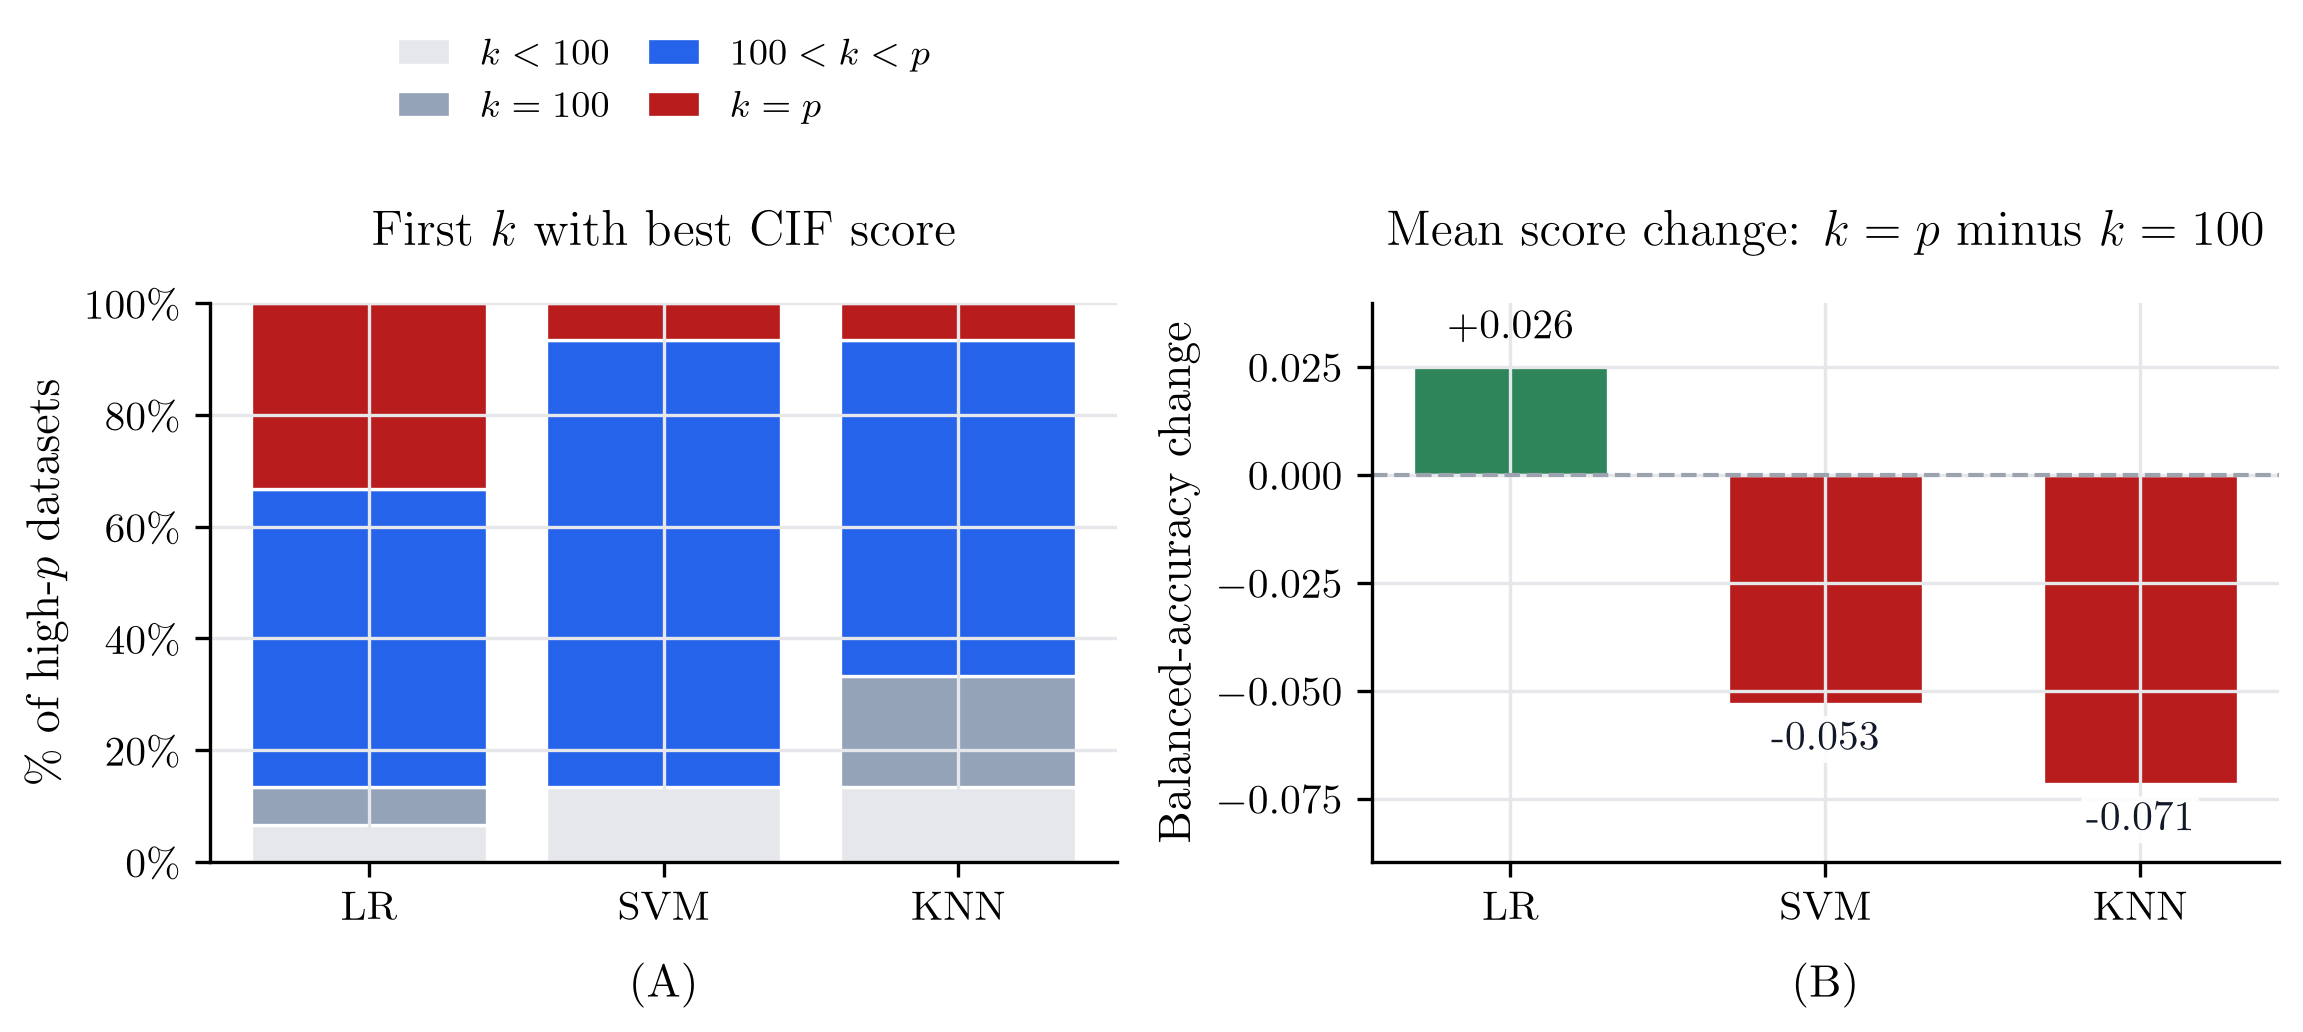
\includegraphics[width=0.84\linewidth]{figures/high_p_boundary_summary.png}
  \caption{Where CIF's classification scores peak as $k$ increases, by
  downstream learner. (A) shows, for each learner, the percentage of 15
  datasets where the first evaluated $k$ attaining the best observed CIF score
  falls below 100, at 100, between 100 and $p$, or at $k=p$. (B) shows the mean
  balanced accuracy change from $k=100$ to $k=p$.}
  \label{fig:high-p-boundary}
\end{figure}

\subsection{Synthetic recovery}
\label{sec:synthetic-recovery}

On synthetic datasets with known informative features, CIF sits at or below
the median position of the methods run on each task
(\cref{tab:synthetic-head}). It recovers true features within the top-$k$ list
more reliably than it places one first. On the redundant-feature designs,
where correlated copies of informative features count as hits, CIF ranks 1st
of 16 in regression and tied 7th of 15 in classification.
\Cref{fig:synthetic-topk-curves} shows recovery as $k$ grows.

\begin{table}[!htbp]
  \centering
  \footnotesize
  \setlength{\tabcolsep}{6pt}
  \begin{tabular}{@{}lcccc@{}}
    \toprule
    & \multicolumn{2}{c}{Classification} & \multicolumn{2}{c}{Regression} \\
    \cmidrule(lr){2-3}\cmidrule(l){4-5}
    \tablehead{Metric} & {Value} & Rank & {Value} & Rank \\
    \midrule
    Selected features that are informative & 35.3\% & \countfrac{8}{15} & 39.1\% & \countfrac{11}{16} \\
    Top-1 hit rate & 65.5\% & \countfrac{10}{15} & 84.5\% & \countfrac{10}{16} \\
    True or redundant (redundant design only) & 82.4\% & \countfrac{7.5}{15} & 83.8\% & \countfrac{1}{16} \\
    \bottomrule
  \end{tabular}
  \caption{Synthetic feature recovery for CIF. The first row averages, over
  $k = 5, 10, 25, 50$, and $100$, the percentage of selected features that are
  truly informative. The top-1 hit rate is computed at $k=1$. The final row is
  computed and ranked only on the redundant-feature design for each task and
  counts true informative plus redundant features. Ranks are among the 15
  classification and 16 regression methods with synthetic runs; fractional
  ranks indicate averaged ties.}
  \label{tab:synthetic-head}
\end{table}

\begin{figure}[!htbp]
  \centering
  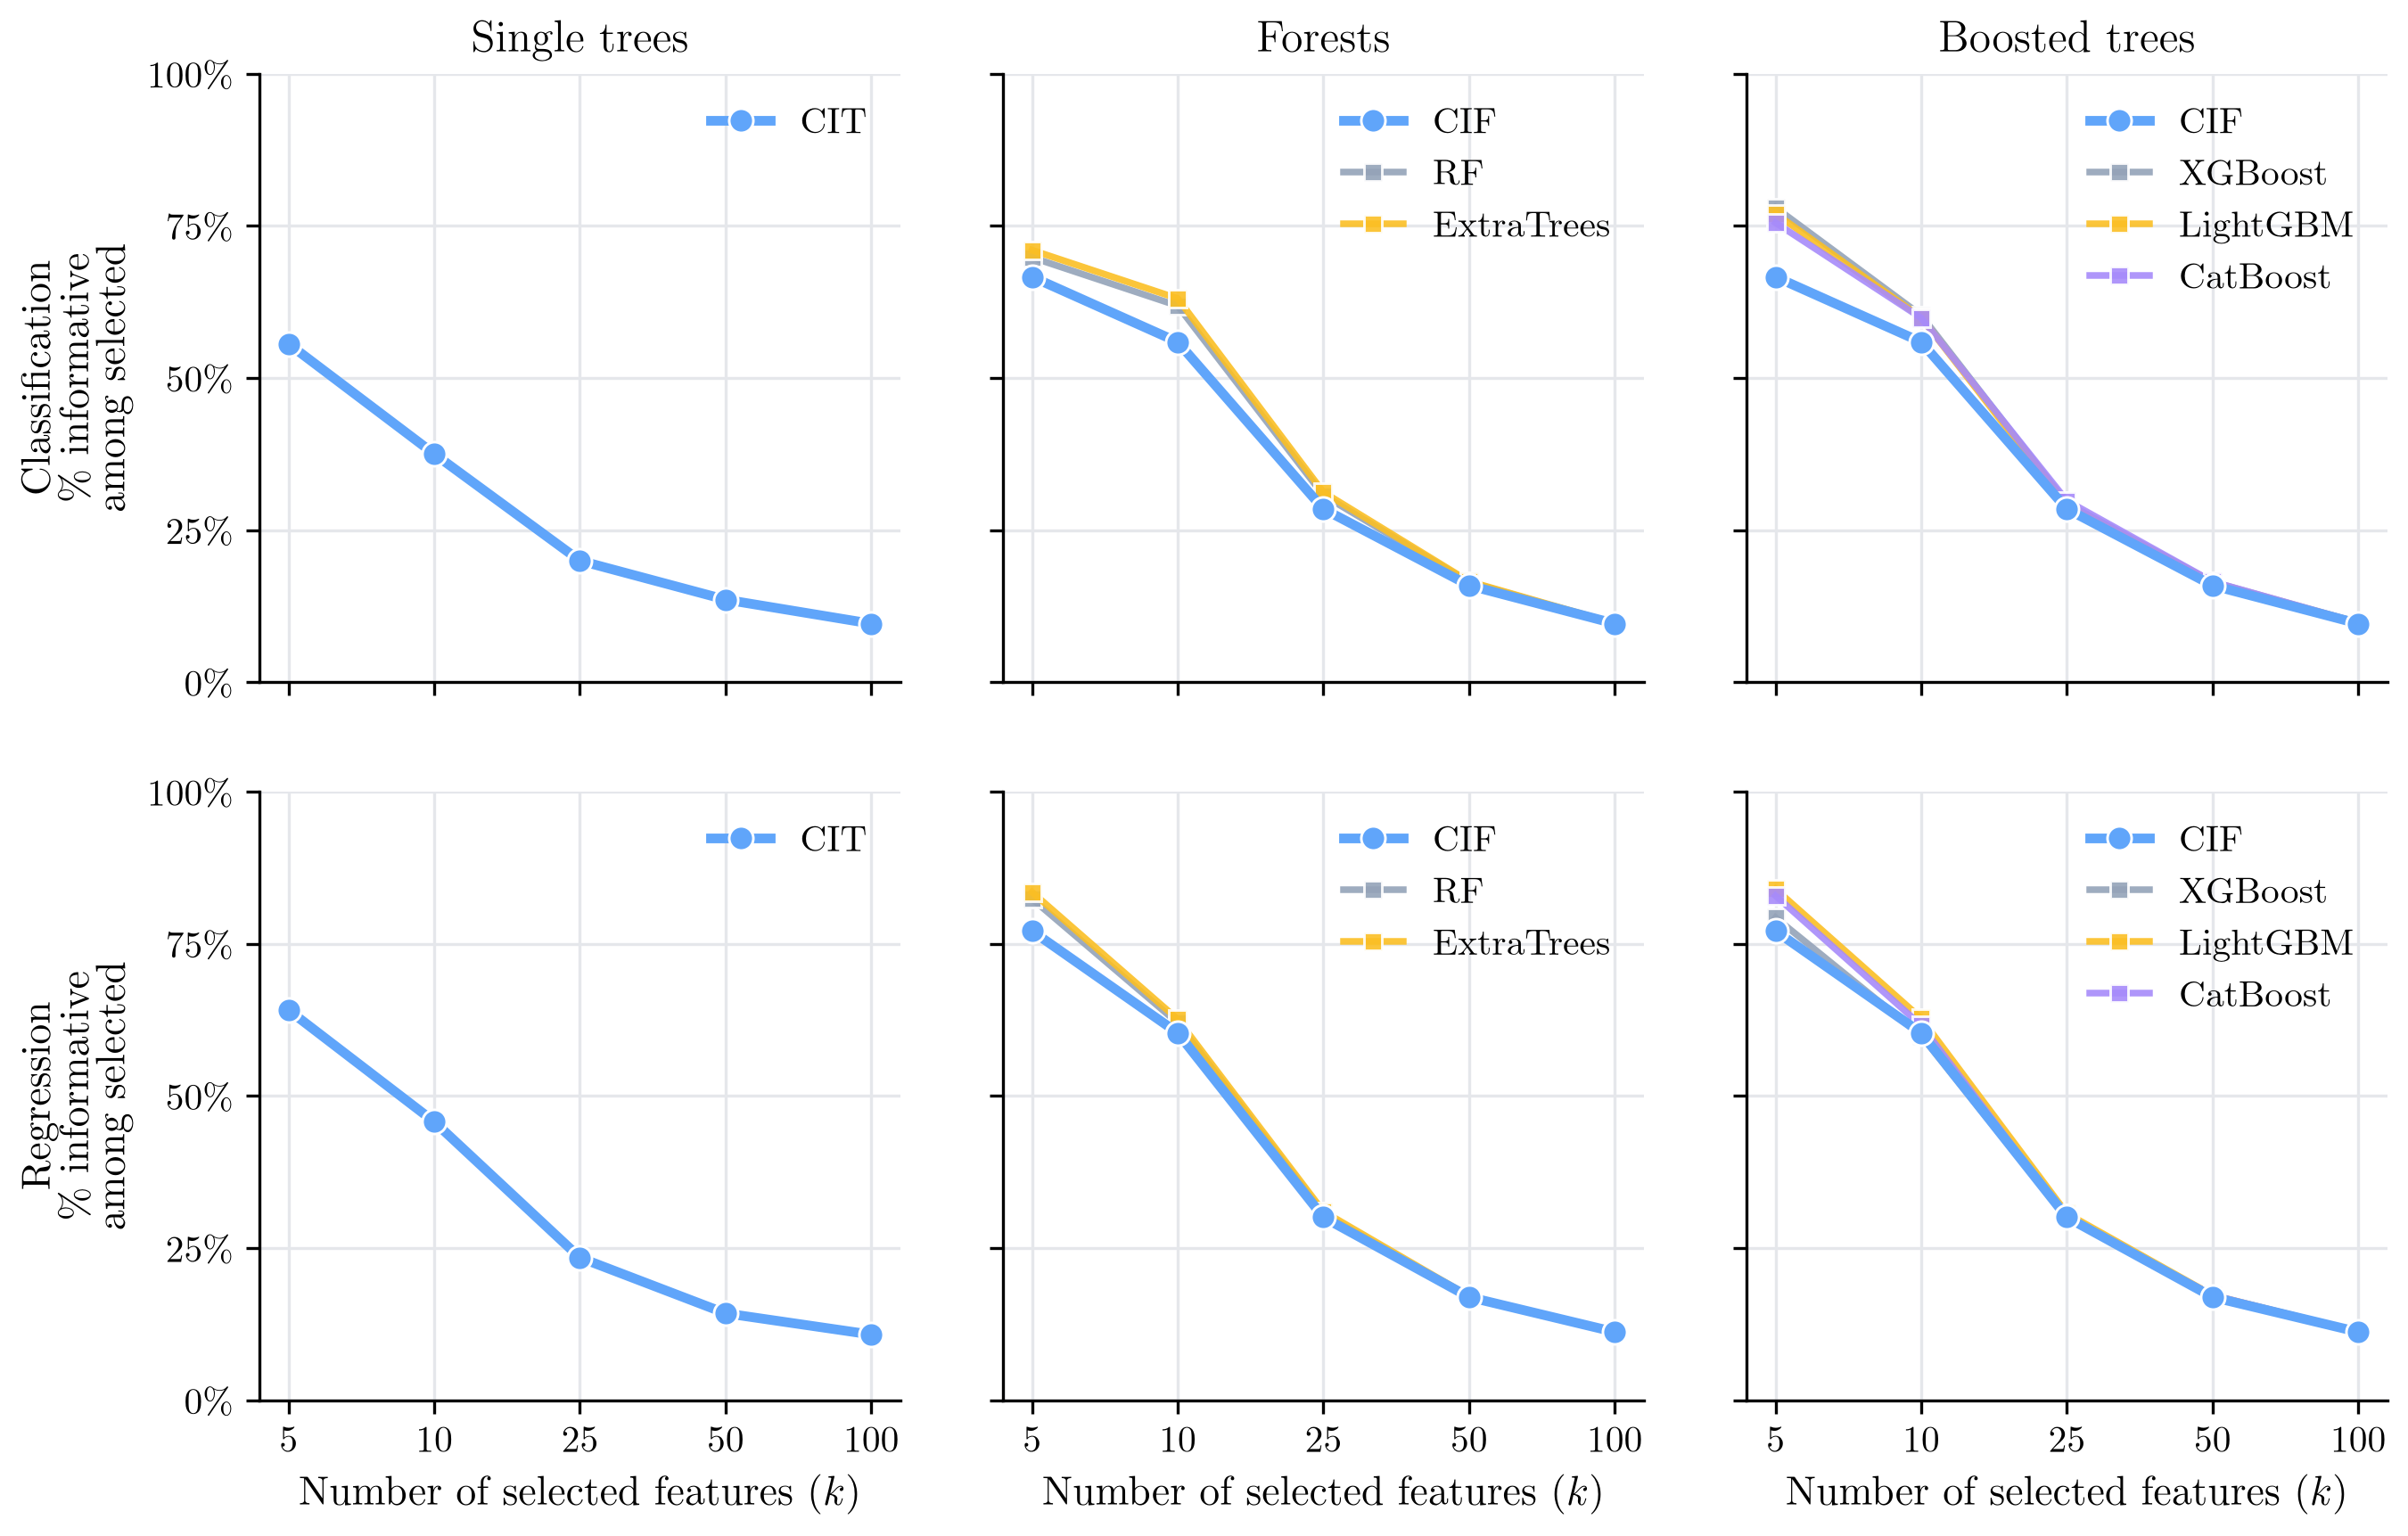
\includegraphics[width=0.84\linewidth]{figures/synthetic_topk_focus_curves.png}
  \caption{Synthetic top-$k$ recovery curves. Columns compare single trees,
  forests, and boosted trees; rows show classification and regression. Each
  value is the percentage of selected features that are truly informative.}
  \label{fig:synthetic-topk-curves}
\end{figure}
